% NOTA: Cada membro do grupo contribuiu 50% para a realização deste relatório

\documentclass[a4paper,12pt]{report}
% PACKAGES  -------------------------------------------------------------------

\usepackage[T1]{fontenc} % Fontes T1
\usepackage[utf8]{inputenc} % Input UTF8
\usepackage[backend=biber, style=ieee]{biblatex} % Para usar bibliografia
\usepackage[portuguese]{babel} % Códigos em PT
\usepackage{lipsum} % Gerar texto automaticamente
\usepackage{graphicx} % Para a inserir imagens
\usepackage{tocbibind} % Criação de indíce
\usepackage{geometry} % Delimitação de margens
\usepackage{parskip} % Incremento de espaço entre parágrafos
\usepackage{multicol}
\usepackage{subfigure} 
\usepackage{hyperref}
\usepackage{csquotes}
\usepackage{url}

% EXTRAS ----------------------------------------------------------------------

\setcounter{tocdepth}{5}
\setcounter{secnumdepth}{5}
\geometry{a4paper,left=2.8cm,right=2.8cm,top=2cm,bottom=3cm}


\begin{document}


% DEFINIÇÕES ------------------------------------------------------------------

\def\titulo{Trabalho de aprofundamento 2} 
\def\data{Abril 2018} 
\def\autores{Francisco Xavier Santos Petronilho, Rui Miguel Silva Oliveira} 
\def\autorescontactos{(89241) franciscoxaviersp@ua.pt, (89216) ruimigueloliveira@ua.pt} 
\def\departamento{DEPARTAMENTO DE ELETRÓNICA, TELECOMUNICAÇÕES E INFORMÁTICA} 
\def\empresa{UNIVERSIDADE DE AVEIRO} 
\def\logotipo{ua.pdf}

% CAPA ------------------------------------------------------------------------

\begin{titlepage} 

\begin{center}

\vspace*{50mm} 

{\Huge\textbf{\titulo}}\\ 
\vspace{13mm} 

{\Large\autores}\\ 
\vspace{15mm}

{\Large \empresa}\\ 
\vspace{10mm} 

\begin{figure}[h]
\center
\includegraphics{\logotipo}
\end{figure}
            
\vspace{30mm} \end{center} 
         

\end{titlepage} 
             
% PÁGINA DE TÍTULO ------------------------------------------------------------

\title{{\Huge\textbf{\titulo}}\\
\vspace{10mm}
{\Large \departamento}\\
\vspace{5mm}
{\LARGE \empresa}} 

\author{\autores \\ \autorescontactos}

\date{\data}

\maketitle
           
\clearpage

\section{Resumo}
Python é sem dúvida uma linguagem extremamente versátil e com a elaboração deste trabalho podemos entender mais profundamente as suas vantagens e a capacidade de resolução de problemas do nosso quotidiano.\par
Inicialmente foi nos proposto criar um cliente com a capacidade de aceder remotamente a uma sonda de temperatura, humidade e vento, sendo que esta possui a capacidade de enviar os dados através de uma rede sem fios. A aquisição é feita de forma automática e constante, emitindo um valor novo a cada 10 segundos.\par
O objetivo do trabalho é registar os dados num ficheiro Comma Separated Values (CSV) e apresentar algumas indicações sobre a necessidade de se levar certas peças de roupa ou acessórios consoante o clima.\par
A comunicação com a sonda é feita através de um socket Transmission Control Protocol (TCP), na porta 8080 do servidor xcoa.av.it.pt, enviando-se comandos de texto e recebendo-se objectos JavaScript Object Notation (JSON).



% ÍNDICE ----------------------------------------------------------------------

\begingroup
\tableofcontents
\endgroup
\clearpage

% LISTA DE FIGURAS ------------------------------------------------------------

\listoffigures
\clearpage



% INTRODUÇÃO ------------------------------------------------------------------

\chapter{Introdução}
\label{introducao}
Qualquer projeto para que seja mais simples de compreender e também metódico na sua resolução do seu todo, terá de ser elaborado de forma faseada. Deste modo, para a resolução do tema que nos foi proposto, inicialmente tivemos que compreender em geral como se processa  comunicação com a sonda, estudando deste modo o que seria um “socket Transmission Control Protocol (TCP)”.\par
A partir podemos tratar da informação que recebíamos do servidor para ser utilizada mais tarde nos métodos de decisão.\par
Por fim foi introduzida a possibilidade de troca de informação com o servidor de forma encriptada.

% DESENVOLVIMENTO -------------------------------------------------------------
\chapter{Desenvolvimento}
\label{desenvolvimento}


\section{Comunicação com a Sonda}
O termo “comunicação”, neste caso com uma sonda, requer além demais conhecimento no que toca a conceitos de comunicação. Assim, para além das aulas onde aprendemos o essencial para conseguir-mos perceber no geral como tudo isto funcionava, tivemos de interiorizar o modelo “Cliente-Servidor”. Mais concretamente foi necessário perceber o que seria um socket e todo o tipo de programação associada ao mesmo. Depois desta ambientação este novo tipo de “programação” foi necessário conhecer a sequência de primitivas utilizadas num Socket TCP.

\vspace{10mm}
\begin{figure}[h]
\center
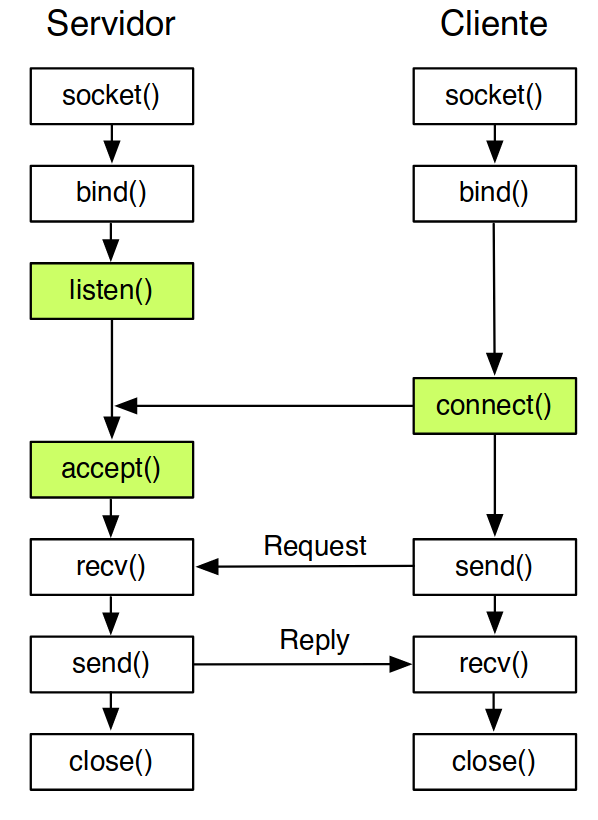
\includegraphics[width=6cm]{imagens/sockettcp.png}
\caption{Sequência de primitivas utilizadas num Socket TCP}
\end{figure}
\clearpage

\section{Tipos de Documentos}
Relembramos que a comunicação com a sonda é feita através de um socket Transmission Control Protocol (TCP), na porta 8080 do servidor xcoa.av.it.pt, enviando-se comandos de texto e recebendo-se objectos JavaScript Object Notation (JSON) e que o objetivo do trabalho é registar dados num ficheiro CSV.\par Assim surgem dois termos novos que que toca à manipulação de documentos em dois formatos muito
comuns, usados para a troca de informação entre aplicações e dispositivos através de sockets, CSV e JSON.\par

\subsection{CSV}
O formato Comma Separated Values CSV é muito comum para a troca de informação especialmente neste tipo de trabalhos onde se troca informações com uma sonda. Um ficheiro CSV é, como o próprio nome indica, é um ficheiro sem formatação em que os valores estão separados por vírgulas, delimitados por aspas e, em que, cada linha tem um registo diferente, ou seja, um artigo, cliente ou fornecedor por linha.
Assim era possível receber os valores da sonda e desta forma serem impressos no terminal.

\subsection{JSON}
O formato JSON assenta basicamente em duas estruturas:\par 
Uma colecção de pares: chave/valor em algumas linguagens de programação tal estrutura é entendida como um objecto, lista, matriz, etc;\par 
Uma lista ordenada de valores nas linguagens de programação é caracterizado como um array, vector, lista, etc;\par
Este tipo de estruturas de dados são transversais a quase todo o tipo de linguagens de programação modernas, o que faz do JSON uma excelente escolha no que se refere ao formato para intercâmbio de informação.\par
De facto é possível converter qualquer estrutura de dicionário ou lista para o formato JSON e vice-versa, o que é extremamente útil para transmitir informação sobre Sockets.\par

Deste modo este formato foi utíl na elaboração do trabalho pois este esta responsável por guardar os valores que interessavam.
\clearpage

\section{Mecanismos de Decisão}
Relembrando o objetivo principal do projeto,  a utilidade pretendida seria a de enviar indicações sobre a possibilidade (ou necessidade) de se levar t-shirt, casaco, gorro ou outras peças de roupa consoante o clima naquele instante de tempo.\par
Deste modo ficou ao critério do grupo criar mecanismos de decisão conforme a humidade a temperatura e o vento. Resumindo sucintamente todas as possibilidades, ficaríamos com 15 mensagens a transmitir no terminal com todas as combinações possíveis das três variáveis anteriormente descritas. Estas seriam:

\vspace{10mm}
\begin{figure}[h]
\center
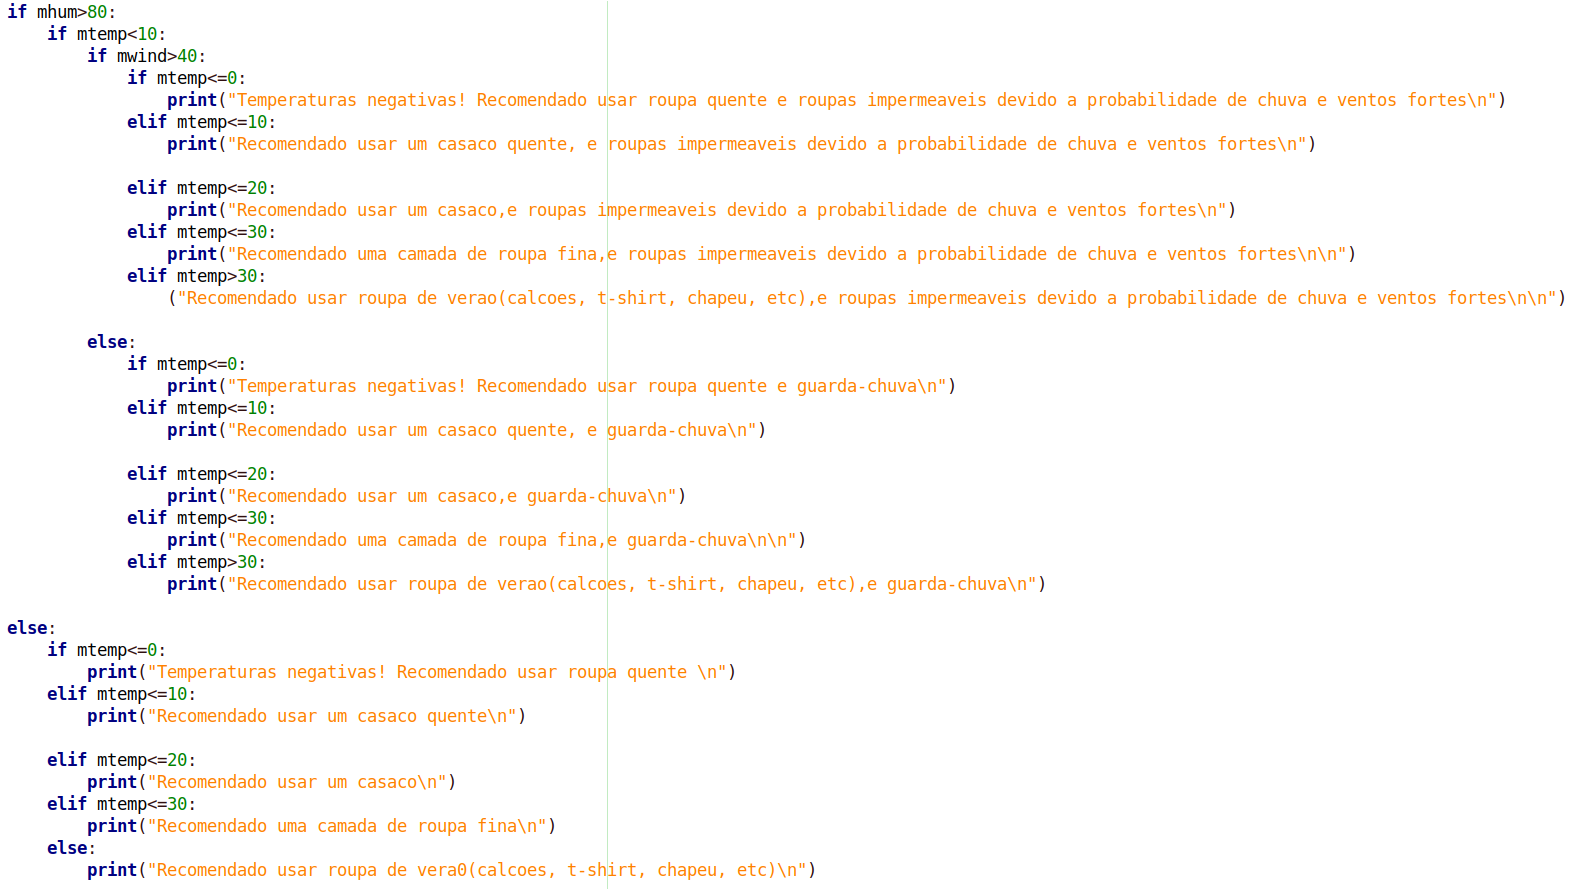
\includegraphics[width=16cm]{imagens/mecdecisao.png}
\caption{Mecanismos de Decisão}
\end{figure}
\clearpage

% CONCLUSÃO -------------------------------------------------------------------
\chapter{Conclusão}
Com a elaboração deste projeto podemos evoluir sigficamente 
\label{conclusão}

\clearpage



% BIBLIOGRAFIA ----------------------------------------------------------------
\begin{thebibliography}{20}

\bibitem{} 
eLearning UA (Laboratŕios de Informática) \\\texttt{https://elearning.ua.pt/course/view.php?id=3470}

\bibitem{} 
PplWare \\\texttt{https://pplware.sapo.pt/tutoriais/json-javascript-objection-notation-o-sucessor-do-xml/}

\end{thebibliography}

\end{document}
